\documentclass[spanish, fleqn]{scrartcl}
\usepackage[utf8]{inputenc}
\usepackage{babel}
\usepackage[paper=a4paper, top=2cm, left=2cm, right=2cm]{geometry}
\usepackage{tikz}
%\usepackage{CIACcustom}
\usepackage{fourier}
\usepackage{amsmath, amsthm}
\usepackage{listings}
\usepackage{multicol}
\usepackage{fancyhdr}
\usepackage[urlcolor=blue, colorlinks]{hyperref}
\usepackage{booktabs,tabularx}
\usepackage{float}

\newcolumntype{L}[1]{>{\hsize=#1\hsize\raggedright\arraybackslash}X}%
\newcolumntype{R}[1]{>{\hsize=#1\hsize\raggedleft\arraybackslash}X}%
\newcolumntype{C}[2]{>{\hsize=#1\hsize\columncolor{#2}\centering\arraybackslash}X}%

\renewcommand{\lstlistingname}{Código}

\pagestyle{fancy}
\fancyhf{}
\rhead{\pgfimage[width=2.5cm]{imagenes/logo-ciac.png}}
\chead{
  Apoyos Intensivos Pauta N°2\\
  IWI-131 Semestre II-2019 \\
  CIAC Casa Central
}
\lhead{\pgfimage[width=2.5cm]{imagenes/logo-usm.jpg}}
\rfoot{\LaTeXe / CIAC 2019}
\lfoot{\thepage}

\renewcommand{\ttdefault}{pcr}

%%% listings settings:
\definecolor{bggray}{rgb}{0.95,0.95,0.95}
\lstdefinestyle{consola}{
  backgroundcolor=\color{bggray},
  basicstyle=\small\ttfamily,
  frame=single,
  moredelim=[is][\bfseries]{[*}{*]},
  xrightmargin=5pt
}

\lstdefinestyle{mypy}{
  language=python,
  backgroundcolor=\color{bggray},
  basicstyle=\ttfamily\small\color{orange!70!black},
  frame=L,
  keywordstyle=\bfseries\color{green!40!black},
  commentstyle=\itshape\color{purple!40!black},
  identifierstyle=\color{blue},
  stringstyle=\color{red},
  numbers=left,
  showstringspaces=false,
  xrightmargin=5pt,
  xleftmargin=10pt
}

\newtheorem{CIACdef}{Definición}

\begin{document}
\vspace*{-.3cm}
\section{La montaña más alta del mundo.}

Michael God y Angel Car, famosos escaladores, programadores y jóvenes empresarios internacionales, sedientos de nuevas aventuras, deciden hacer trabajar a los estudiantes de programación que van a los intensivos del CIAC para saber cual es la montaña más alta que han escalado.
\\ \\
La información de sus aventuras la guardan en una lista de tuplas con el nombre \texttt{montanas} que tiene el formato \texttt{nombre,altura,hora\_inicio,hora\_fin}, donde \texttt{nombre} es un string, \texttt{altura} es un entero en metros y los datos restantes son tuplas de la forma \texttt{(horas,minutos)}.
\\
\begin{lstlisting}[style=consola]
montanas=[
    ('Nielol',335,(14,00),(17,35)),
    ('La Campana',1880,(8,4),(17,34)),
    ('Churen Himal',7385,(5,34),(23,14)),
    ('Everest',8848,(8,23),(10,43)), #fue en helicoptero
    ('Mont Blanc',4810,(4,12),(21,45)),
    #...
    ('Kilimanjaro',5895,(12,15),(19,31))
    ]

\end{lstlisting}
\\
Ellos quieren que los estudiantes programen las siguientes funciones

\begin{itemize}
    \item \texttt{filtro\_altura\_nombre(montanas)} que reciba la lista \texttt{montanas} y retorne una lista de tuplas con la altura y el nombre ordenadas de menor a mayor.
    \\
    \begin{lstlisting}[style=consola]
>>> filtro_altura_nombre(montanas)
[(335, 'Nielol'), (1880, 'La Campana'), (4810, 'Mont Blanc'), 
(5895, 'Kilimanjaro'), (7385, 'Churen Himal'), (8848, 'Everest')]
    \end{lstlisting}

    \item \texttt{duracion(inicio,fin)} que reciba dos tuplas con la hora de inicio y fin y retorne una tupla de la forma \texttt{hora,minutos} con la duración de la escalada
    \\
    \begin{lstlisting}[style=consola]
>>> duracion((14,0),(17,35))
(3, 35)
    \end{lstlisting}
    \item Finalmente escriba un programa que indique cual fue la montaña más alta que escalaron, la altura en metros que tenía y el tiempo empleado. La información que se muestra por pantalla debe tener la siguiente forma
    \begin{lstlisting}[style=consola]
La montana mas alta que escalaron fue Everest.
Esta tenia una altura de 8848 metros.
Se demoraron 2 horas y 20 minutos.
    \end{lstlisting}
    
\end{itemize}
\section{¡Triángulos!... ¿Otra vez?}

A continuación de presenta una posible implementación de la función pedida (¿Alguien lee esta parte?):
  
\lstinputlisting[
    style  = mypy,
    caption= \texttt{pascal.py}]{Code/p2.py}

\section{Una de archivos de texto}

A la universidad Santa María, lider en ingeniería, magia y hechicería, llegan alumnos de intercambio provenientes de Hogwarts para tomar el curso de defensa contra las artes oscuras. Los profesores (magos) son nulos en el manejo de datos y le piden a los buenos estudiantes de IWI-131 (muggles) que van a los intensivos de CIAC ayuda con el filtro de alumnos aprobados y reprobados. Las reglas para aprobar son:
\begin{itemize}
    \item Que el promedio de sus notas sea mayor o igual a 55.
    \item Que el porcentaje de asistencia sea mayor al 75\%
\end{itemize}

De cumplirse ambas condiciones, el estudiante aprueba, de cumplirse sólo una, el estudiante debe dar un examen global y de no cumplirse ninguna el estudiante reprueba.

Se tienen los archivos: notas.txt y asistencia.txt

\begin{figure}[h]
    \centering
    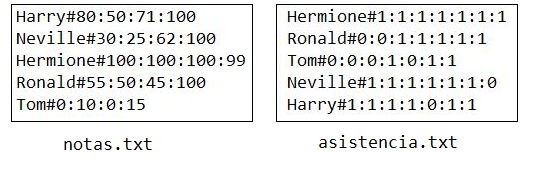
\includegraphics[scale=0.9]{Imagenes/archivos1.jpg}
\end{figure}

El archivo notas.txt tiene la estructura \texttt{nombre\_alumno\#nota1: ... :nota4}, mientras que el archivo asistencia.txt tiene la estructura \texttt{nombre\_alumno\#asis1: ... :asis7}. A usted se le pide:

\begin{itemize}
    \item[a.] Desarrollar la función \texttt{listado\_alumnos(nombre\_archivo)} que reciba como parámetro el nombre de uno de los dos archivos y retorne una lista con todos los alumnos.
    \begin{lstlisting}[style=consola]
>>>listado_alumnos('notas,txt')
['Harry','Neville','Hermione','Ronald','Tom']
    \end{lstlisting}
    \item[b.] Desarrollar la función \texttt{aprueba\_por\_notas(nombre\_archivo)} que reciba como parámetro el nombre del archivo con las notas y retorne un diccionario que asocie el nombre del alumno con un booleano según haya o no cumplido con el requisito número 1.
    \begin{lstlisting}[style=consola]
>>>aprueba_por_notas('notas.txt')
{'Ronald':True,'Neville':False,'Harry':True,'Hermione':True,'Tom':False}
    \end{lstlisting}
    \item[c.] Programar la función \texttt{aprueba\_por\_asistencia(nombre\_archivo)} que reciba como parámetro el nombre del archivo con las asistencias y retorne un diccionario que asocie el nombre del alumno con un booleano según haya o no cumplido con el requisito número 2.
    \begin{lstlisting}[style=consola]
>>>aprueba_por_asistencia('asistencia.txt')
{'Ronald':False,'Neville':True,'Harry':True,'Hermione':True,'Tom':False}
    \end{lstlisting}
    \item[d.] Crear la función \texttt{resumen(archivo\_notas,archivo\_asistencia)} que reciba los nombres de ambos archivos, y cree el archivo \texttt{Final.txt} con la estructura \texttt{nombre\#estado}, donde estado puede ser (APROBADO, EXAMEN GLOBAL, REPROBADO) de cada alumno. La función retorna None.
    \begin{figure}[h]
    \centering
    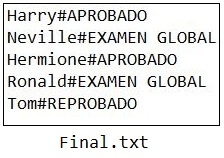
\includegraphics[scale=0.9]{Imagenes/final.jpg}
    \end{figure}
\end{itemize}
\section{Notas, archivos y ¿diccionarios?}

Considerando el mismo formato de la pregunta anterior, cree las siguientes funciones:

\begin{itemize}
    %%% Se necesitaron 4 cabezas para pensar en esta palabra.
    \item \texttt{diccioinador(archivo)}. Esta función recibe el nombre de un archivo con el formato entregado en la pregunta anterior. 
    
    Retorna un diccionario, donde las llaves son el nombre de las personas, y el valor es un diccionario de ramos de dicho estudiante. La llave de esta diccionario es la sigla de un ramo, y la llave es una tupla con las notas de este ramo como enteros (no se considera el promedio de notas).
    
    \begin{lstlisting}[style=consola]
>>> [*dicc = diccioinador("notas.txt")*]
>>> [*print(dicc)*]
{'anghelo': {'mat021': (76, 78, 54)}, 
 'miguel': {'mat021': (80, 56, 67), 'fis100': (95, 86, 75)}, 
 'diego': {'iwi131': (100, 99, 98)}
 }
    \end{lstlisting}
    
    \item \texttt{archivinador(archivo, diccionario)}. Esta función recibe el nombre de un archivo y el diccionario antes descrito. 
    
    Esta función escribe en el archivo los datos del diccionario, respetando la estructura del archivo antes descrito.
    
    \begin{lstlisting}[style=consola]
>>> [*dicc = archivinador("notas2.txt", dicc)*]
>>> 
    \end{lstlisting}
    
\begin{center}
\begin{tabular}{|l|}
    \hline
    \texttt{notas2.txt} \\ 
    \hline
    miguel\#mat021\#80;56;67 \\
    miguel\#fis100\#95;86;75 \\
    anghelo\#mat021\#76;78;54 \\
    diego\#iwi131\#100;99;98 \\
    \hline
\end{tabular}
\end{center}
    
    \item \texttt{agregar\_alumno\_inador(archivo, nombre, ramos)}. Esta función recibe el nombre de un archivo con la estructura antes dada, un string con el nombre de un alumno y un diccionario, donde las llaves del diccionario son las siglas de los ramos, y las llaves son una tupla con las notas de dicho estudiante.
    
    Esta función agrega los ramos en el diccionario \texttt{ramos} de estudiante \texttt{nombre} al archivo en cuestión. Si el estudiante ya tenia ese ramo, entonces se debe reemplazar las notas de ese ramo en el archivo.
    
    Lógicamente, si el estudiante no existía en el archivo anteriormente, debe ser agregado.
    
    \begin{lstlisting}[style=consola]
>>> [*ramos = {"iwi131": (42, 69, 90), "fis100": (51, 63, 54)}*]
>>> [*agregar_alumno_inador("notas2.txt", "anghelo", ramos)*]
>>> 
    \end{lstlisting}

\begin{center}
\begin{tabular}{|l|}
    \hline
    \texttt{notas2.txt} \\ 
    \hline
    anghelo\#mat021\#76;78;54 \\
    anghelo\#iwi131\#42;69;90 \\
    anghelo\#fis100\#51;63;54 \\
    miguel\#mat021\#80;56;67 \\
    miguel\#fis100\#95;86;75 \\
    diego\#iwi131\#100;99;98 \\
    \hline
\end{tabular}
\end{center}
\end{itemize}

\end{document}